\chapter{METODE TUGAS AKHIR}

\section{Alat dan Bahan Tugas Akhir}
\subsection{Alat Tugas Akhir}
Pada penelitian ini dibutuhkan beberapa alat. Alat tersebut dapat berupa perangkat keras ataupun perangkat keras. Adapaun alat dalam bentuk perangkat keras yang digunakan dalam penelitian ini adalah sebagai berikut
\begin{enumerate}
	\item Apple MacBook Pro dengan prosesor Apple M1 Pro 16-\textit{core} dan memori terpadu 16 GB dengan sistem operasi macOS Ventura versi 13.2.1 (22D68)
	\item Silicon Labs CP2102 USB \textit{to} TTL \textit{converter} untuk menghubungkan modul Teseo-LIV3FL dengan komputer
	\item \textit{Multimeter} untuk mengukur arus yang digunakan oleh modul Teseo-LIV3FL
\end{enumerate}
Selanjutnya, alat dalam bentuk perangkat lunak yang diunakan adalah sebagai berikut
\begin{enumerate}
	\item STM32CubeIDE sebagai IDE untuk mengunggah program ke mikrokontroler STM32 Nucleo-WL55JC1
	\item STM32Cube Programmer untuk mengunggah \textit{firmware} yang telah di-\textit{build} menggunakan STM32Cube IDE
	\item Pustaka \textit{hardware abstraction layer} (HAL) untuk STM32 WLxx versi 1.3.0
	\item \textit{Driver} BSP untuk Teseo-LIV3FL oleh STMicroelectronics
	\item Aplikasi Teseo-Suite untuk mengunggah konfigurasi dan meninjau konstelasi yang digunakan oleh modul GNSS lebih lanjut
	\item CoolTerm untuk meninjau dan mencatat pembacaan dari \textit{serial port}
	\item Jupyter Notebook untuk analisis dan visualisasi data
\end{enumerate}

\subsection{Bahan Tugas Akhir}
Bahan-bahan yang digunakan dalam penelitian ini adalah sebagai berikut:
\begin{enumerate}
	\item STM32 Nucleo-WL55JC1 berbasis ARM Cortex-M0 dan ARM Cortex-M4 sebagai mikrokontroler pada \textit{end-node}
	\item Modul GNSS Teseo-LIV3FL untuk melacak posisi dari sistem berdasarkan berbagai konstelasi satelit
	\item Antena Taoglas CGGP.18.2.A.02 sebagai penangkap isyarat GNSS untuk kemudian diolah oleh modul Teseo-LIV3FL
	\item Kabel USB \textit{to} \textit{micro} USB untuk menghubungkan \textit{development board} STM32 Nucleo-WL55JC1 dengan komputer
	\item Kabel \textit{jumper} untuk menghubungkan modul Teseo-LIV3FL dengan \textit{development board} STM32 Nucleo-WL55JC1
\end{enumerate}
Selain itu, data yang digunakan dalam penelitian ini mengacu pada standar NMEA-0813.

\section{Alur Tugas Akhir}
Penelitian ini dilakukan dengan melalui beberapa tahapan. Diagram alir dari tahapan penelitian ini ditunjukan oleh Gambar \ref{Fig: diagram-alir-penelitian}. Alur penelitian diawali dengan melakukan studi literatur, perancangan perangkat keras, konfigurasi modul GNSS Teseo-LIV3FL, pengembangan \textit{firmware} pada STM32 Nucleo-WL55JC1, dan diakhiri dengan penyusunan laporan akhir.

\begin{figure}[H]
	\centering
	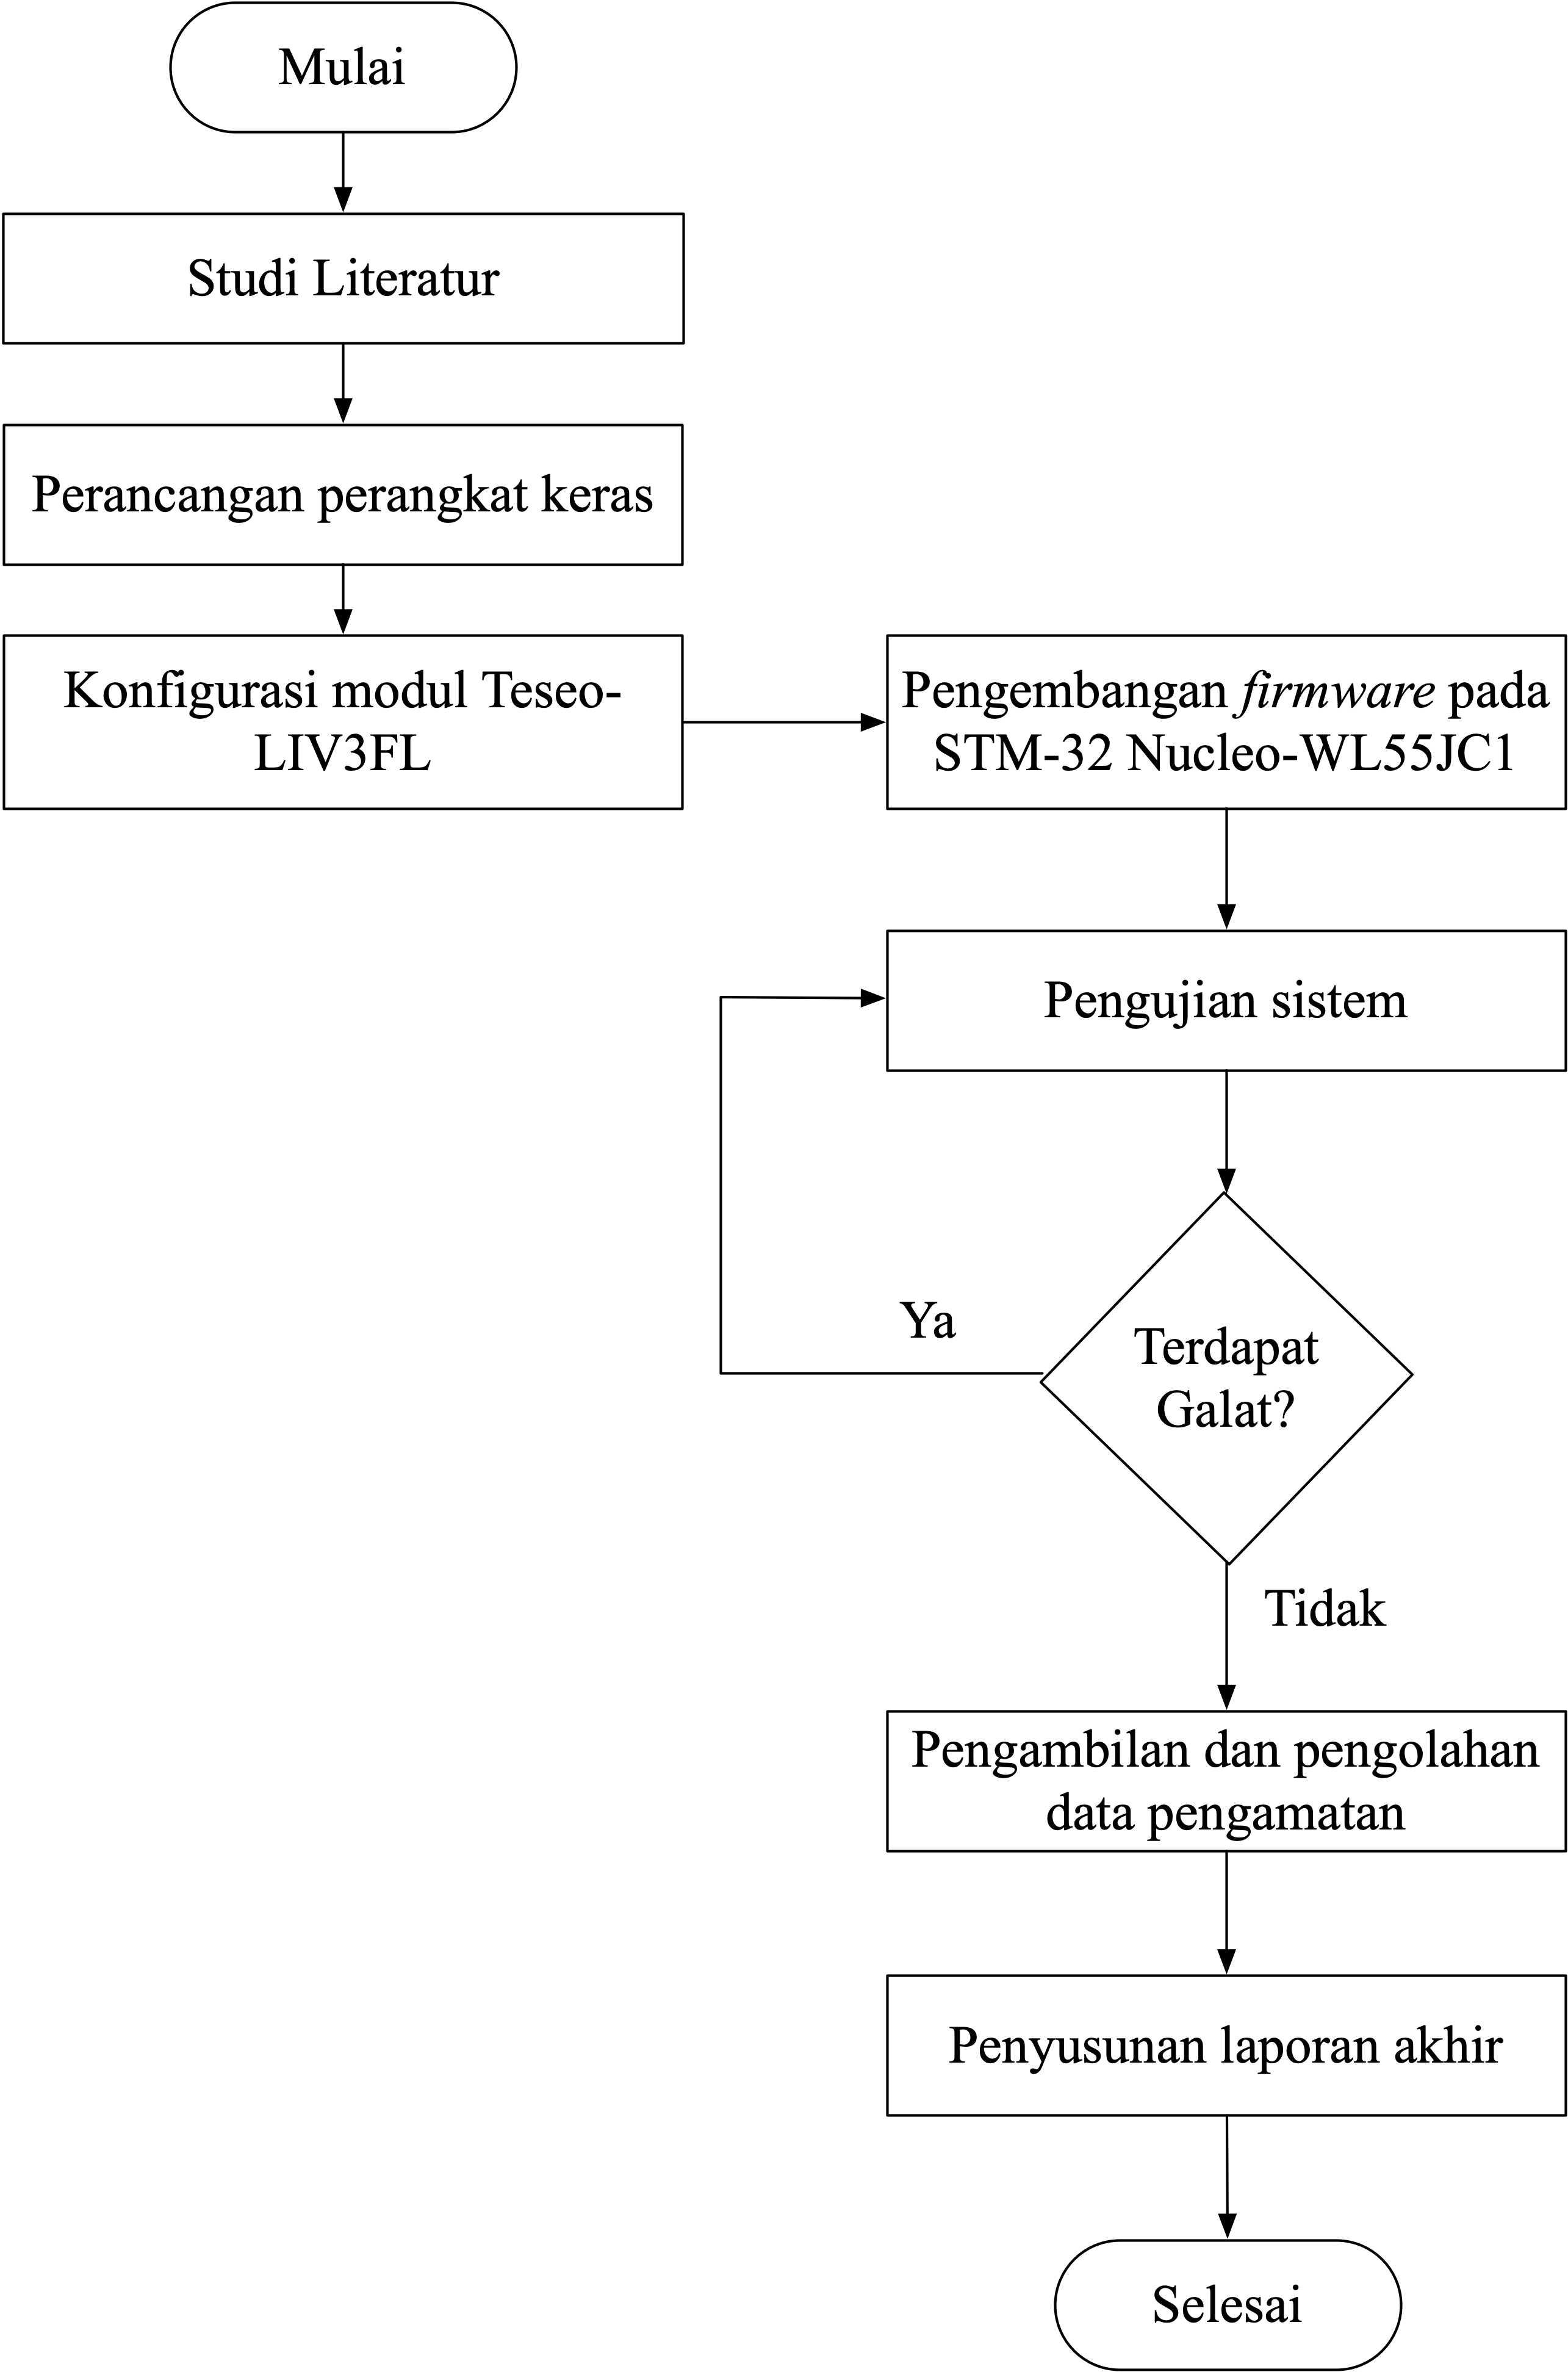
\includegraphics[width=10.5cm]{contents/chapter-3/diagram-alir-penelitian.png}
	\caption{Diagram Alir Penelitian}
	\label{Fig: diagram-alir-penelitian}
\end{figure}

\section{Studi Literatur}
Studi literatur dilakukan dengan mengumpulkan berbagai materi sebagai acuan dalam melakukan penelitian. Referensi tersebut meliputi artikel dan jurnal ilmiah, laporan penelitian sebelumnya, situs web, dan dokumentasi perangkat yang digunakan. Tahapan ini dilakukan dengan tujuan memperoleh gambaran latar belakang, landasan teori yang digunakan dalam penelitian, dan keahlian mengenai topik penelitian.

\section{Perancangan Perangkat Keras}
Dalam penelitian ini, dilakukan perancangan secara garis besar berdasarkan analisis kebutuhan sistem. Rancangan purwarupa sistem digambarkan oleh  Gambar \ref{Fig: system-overview}. Fokus penelitian ini adalah pada perancangan \textit{firmware} di STM32 saja.

\begin{figure}[H]
	\centering
	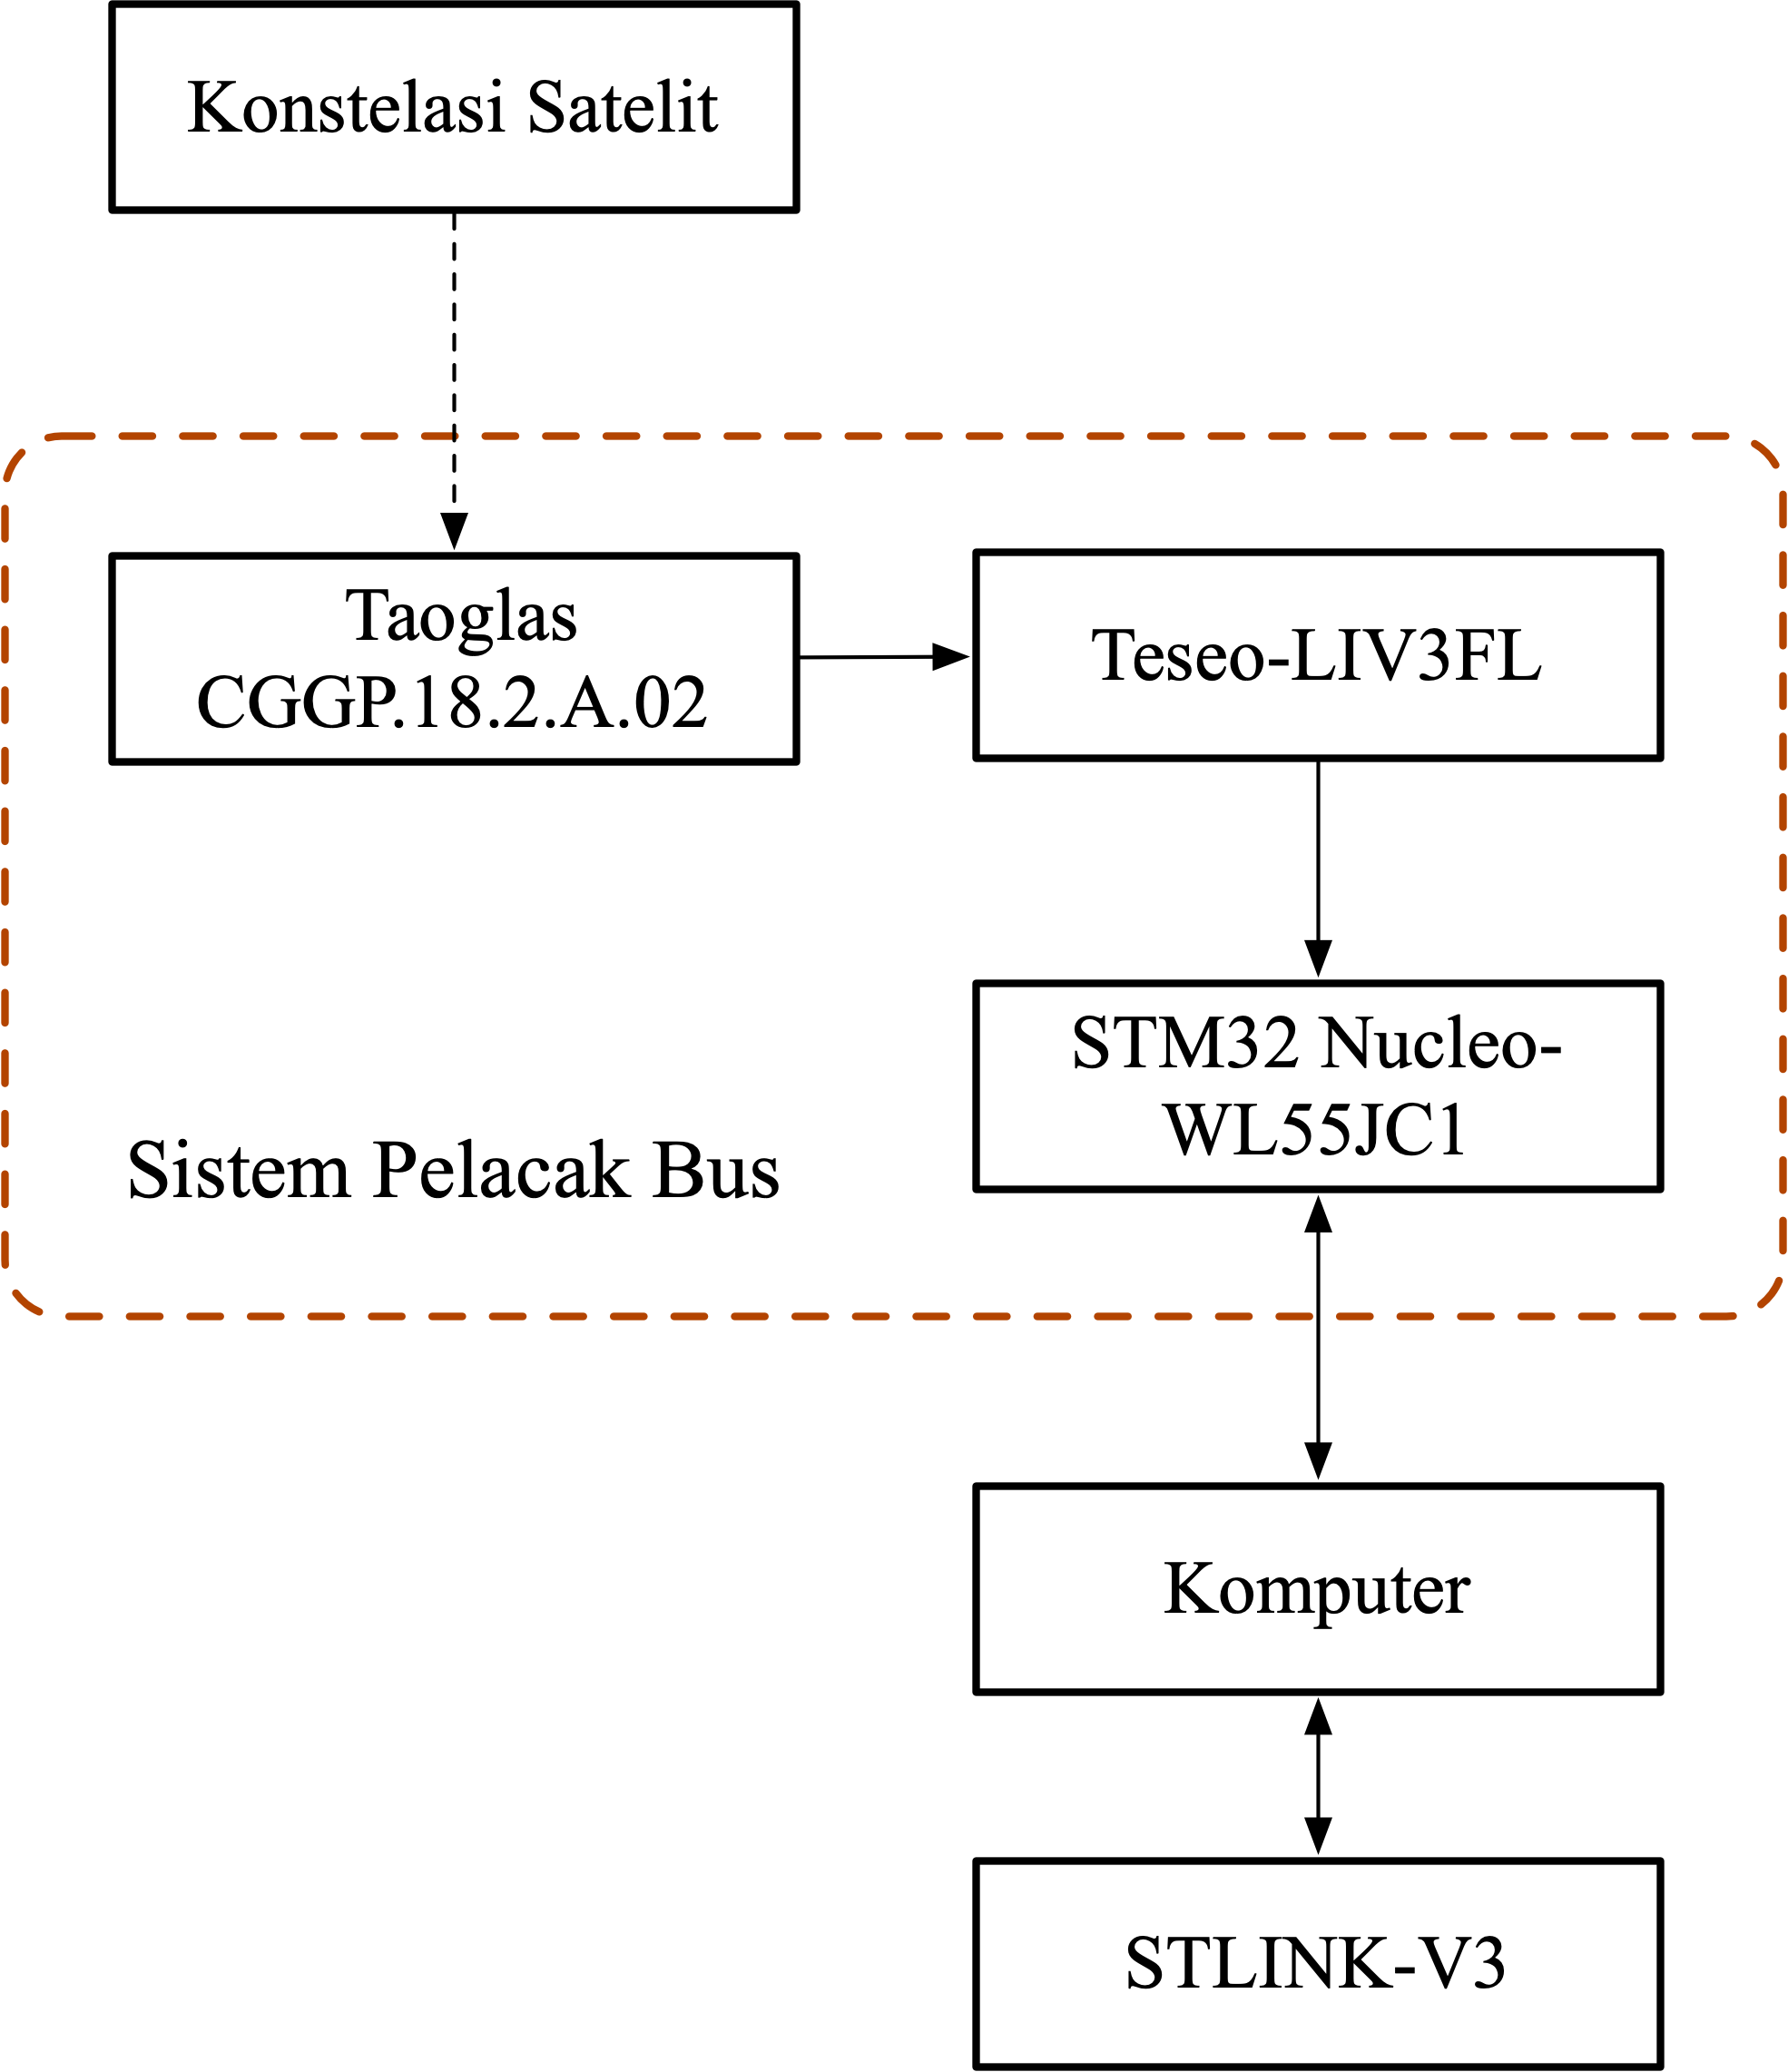
\includegraphics[width=9cm]{contents/chapter-3/system-overview.png}
	\caption{Ikhtisar Sistem}
	\label{Fig: system-overview}
\end{figure}

Modul GNSS yang digunakan adalah Teseo-LIV3FL milik STMicroelectronics. Komunikasi antara modul Teseo-LIV3FL dengan mikrokontroler menggunakan protokol UART dengan \textit{baud rate} 9600 bps. Protokol UART dipilih karena implementasinya yang sederhana. 

\textit{Development board} yang digunakan adalah STM32 Nucleo-WL55JC1 dengan mikrokontroler STM32WL55. \textit{Development board} ini sudah terintegrasi dengan STLINK-V3 sehingga untuk mengunggah \textit{firmware} dapat dilakukan langsung dengan menggunakan \textit{micro} USB pada \textit{development board}.

Untuk dapat menentukan posisi, modul Teseo-LIV3FL perlu untuk mengetahui informasi satelit. Informasi tersebut didapat dari isyarat GNSS yang ditangkap oleh antena. Adapun antena yang digunakan pada penelitian ini adalah \textcolor{red}{Abracon XXX}. 

Pada penelitian ini, modul Teseo-LIV3FL dan antena \textcolor{red}{Abracon XXX} sudah disolder dalam satu papan yang disediakan oleh PT Lunar Inovasi Teknologi. Purwarupa dari perangkat keras ditunjukan oleh Gambar \ref{Fig: purwarupa-alat}

\begin{figure}[H]
	\centering
	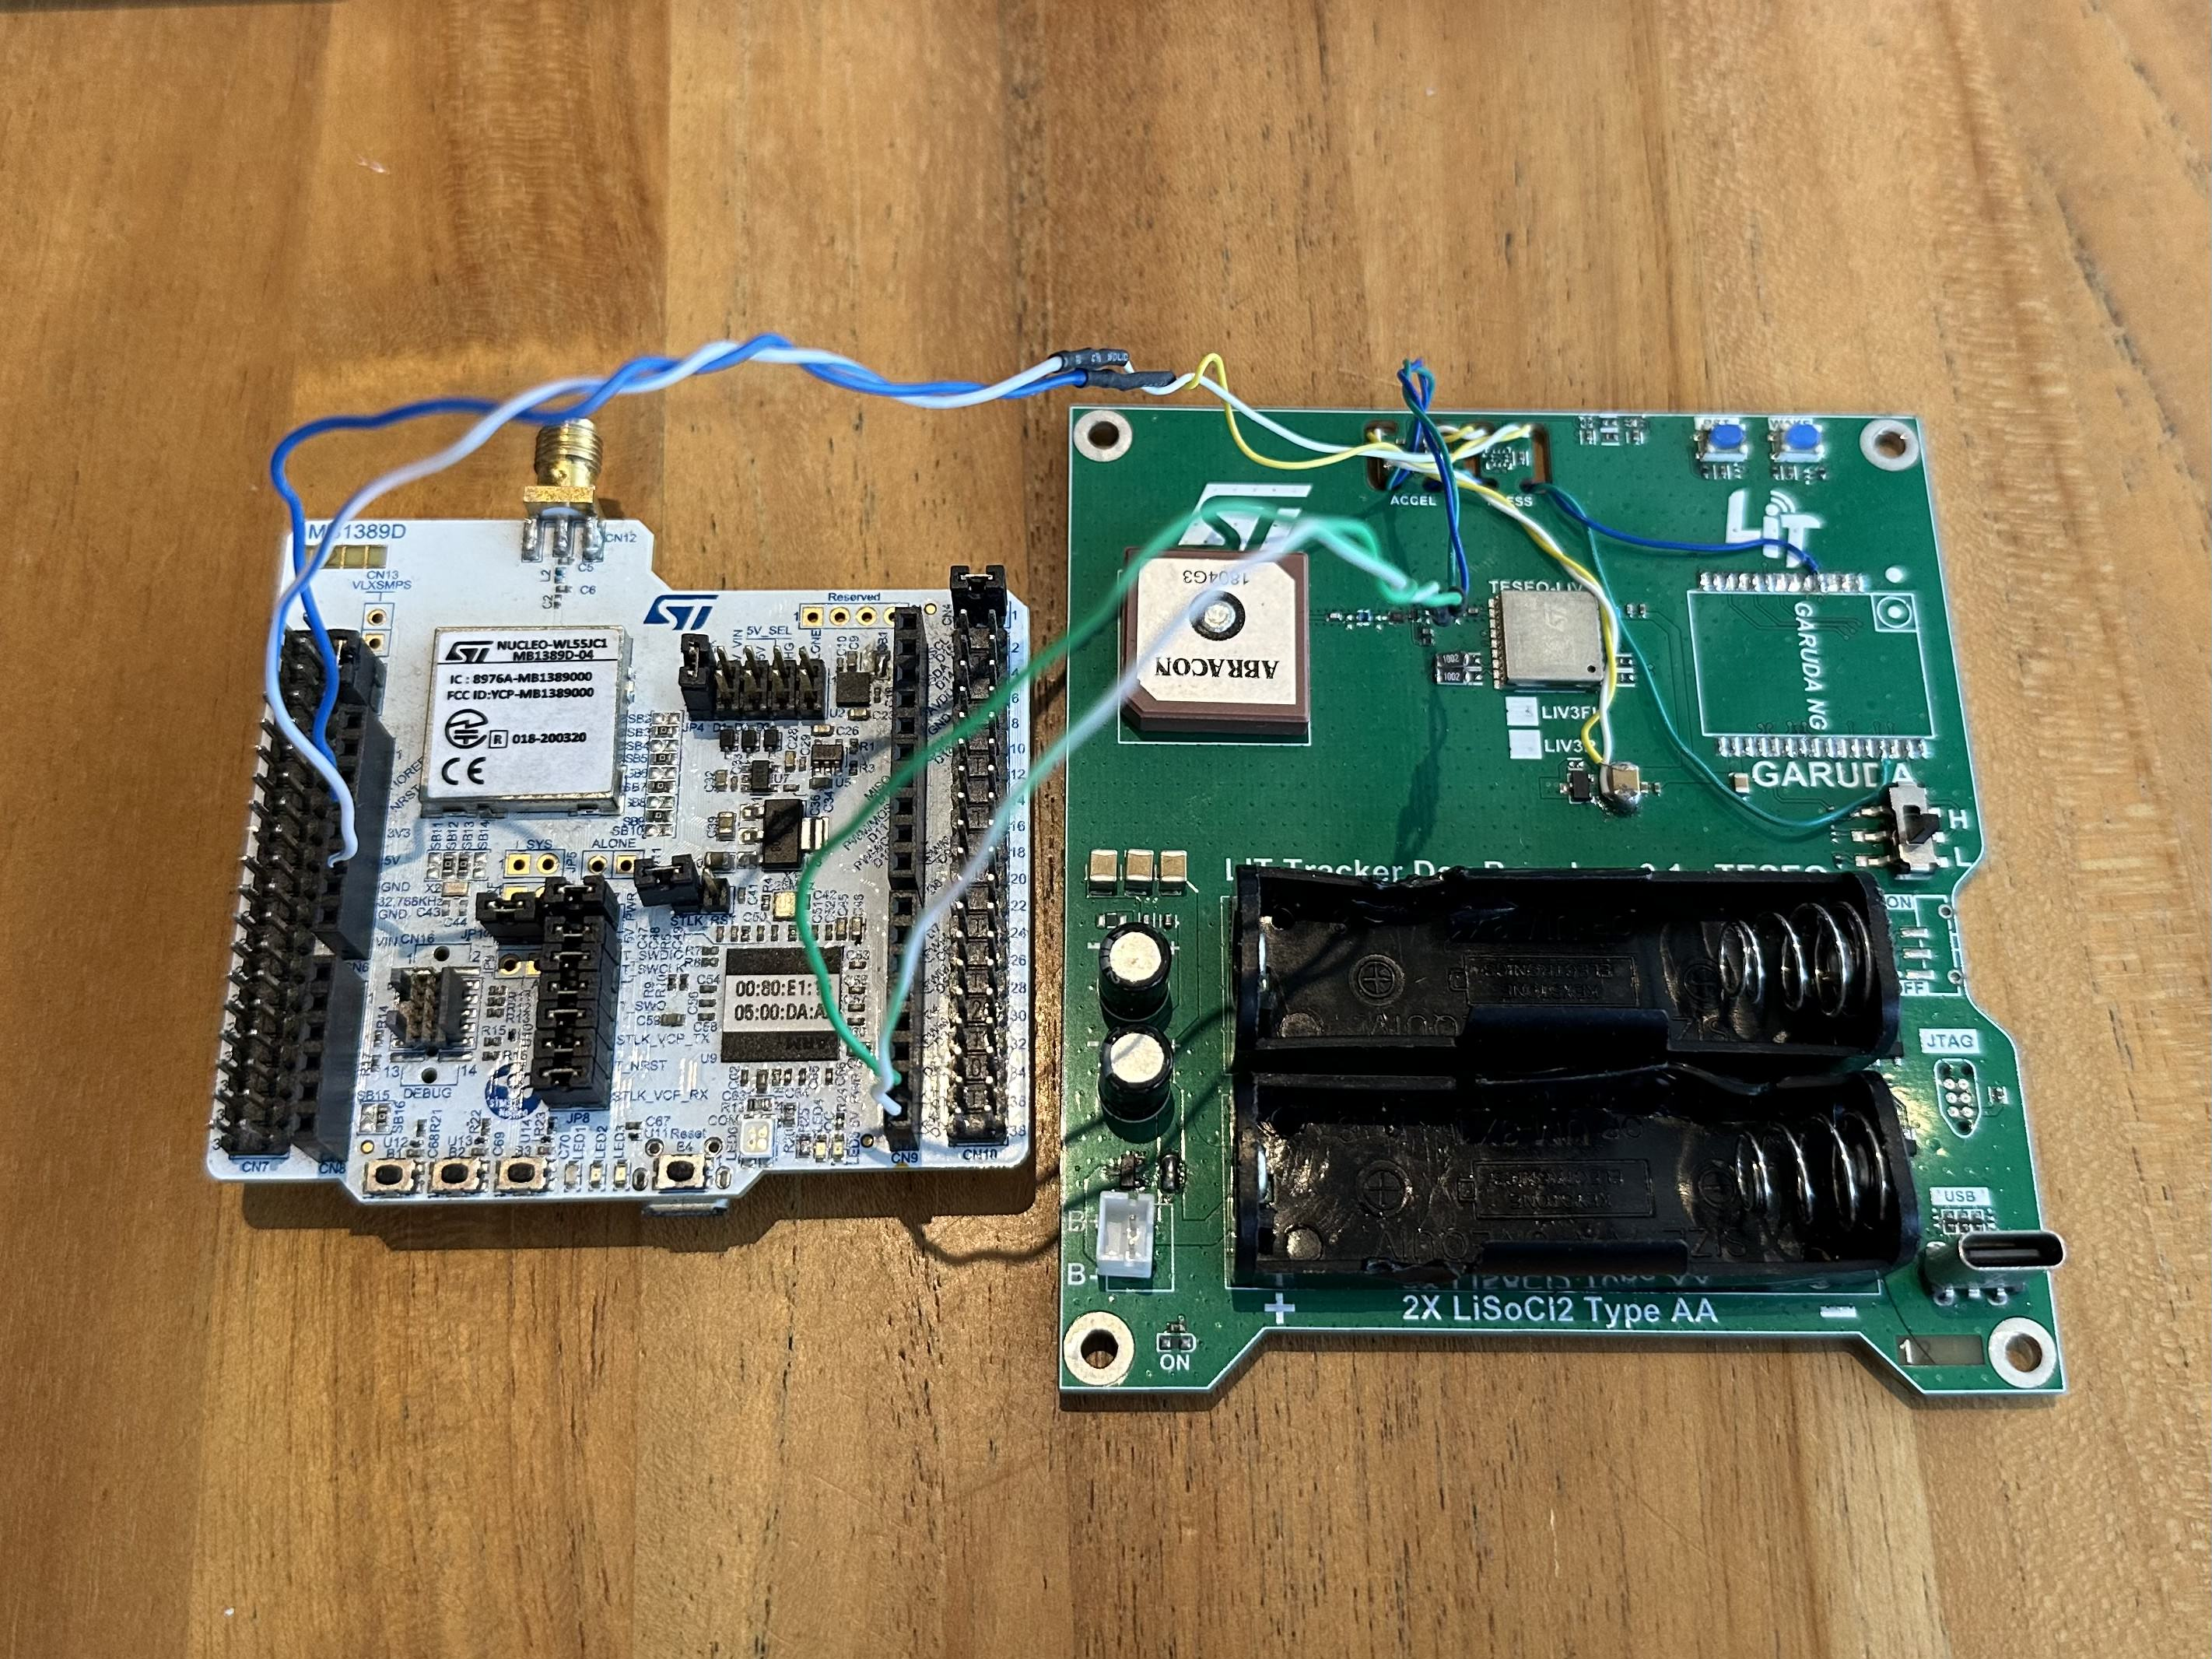
\includegraphics[width=9cm]{contents/chapter-3/purwarupa.jpg}
	\caption{Purwarupa Perangkat Keras}
	\label{Fig: purwarupa-alat}
\end{figure}

\section{Konfigurasi pada Modul Teseo-LIV3FL}
Konfigurasi pada modul Teseo-LIV3FL dikelompokan dalam suatu blok data dengan setiap blok memiliki tiga digit ID. Digit pertama pada setiap ID merepresentasikan tipe parameter dan dua digit lainnya untuk membedakan parameter lainnya dalam tipe tersebut. Ketika sistem berjalan terdapat tiga kemungkinan \textit{configuration block} yang akan dijalankan:
\begin{enumerate}
	\item \textbf{Konfigurasi saat ini} berisi konfigurasi dari setiap blok saat ini disimpan pada RAM. Ketika modul diaktifkan ia akan memuat konfigurasi yang tersimpan pada \textit{non-volatile memory} (NVM) atau konfigurasi bawaan pabrik yang tertanam.
	\item \textbf{Konfigurasi bawaan} disimpan pada \textit{read only memory} (ROM). Konfigurasi ini akan dimuat ketika tidak ada konfigurasi valid pada NVM.
	\item \textbf{Konfigurasi NVM} berisi parameter yang telah dimodifikasi dan disimpan oleh pengguna.
\end{enumerate}

Selain konfigurasi dengan CDB, modul Teseo-LIV3FL juga menawarkan konfigurasi dengan \textit{firmware configuration command}. \textit{Firmware configuration command} memungkinkan pengguna untuk mengatur berbagai CBD-ID dengan satu perintah saja.

\subsection{Konfigurasi \textit{Multi-constellation}}
Modul Teseo-LIV3FL memiliki kemampuan untuk menerima isyarat dari lebih dari satu konstelasi GNSS. Kemampuan tersebut biasa dikenal sebagai \textit{multi-constellation}. Fitur ini dapat memperbaiki akurasi dari modul GNSS jika dibandingkan dengan menggunakan isyarat dari satu konstelasi saja \cite{An2020}.

Untuk mempermudah proses konfigurasi konstelasi maka digunakan aplikasi Teseo-Suite untuk mengunggah konfigurasi ke \textit{non-volatile memory} pada modul Teseo-LIV3FL. Aplikasi Teseo-Suite memiliki fitur untuk meninjau isyarat GNSS yang diterima dan digunakan. Isyarat yang digunakan oleh modul Teseo-LIV3FL sebelum dilakukan konfigurasi ditunjukan oleh Gambar \ref{Fig: sebelum-konfigurasi}. Terlihat bahwa konstelasi yang digunakan hanya GPS.
 
 \begin{figure}[H]
 	\centering
 	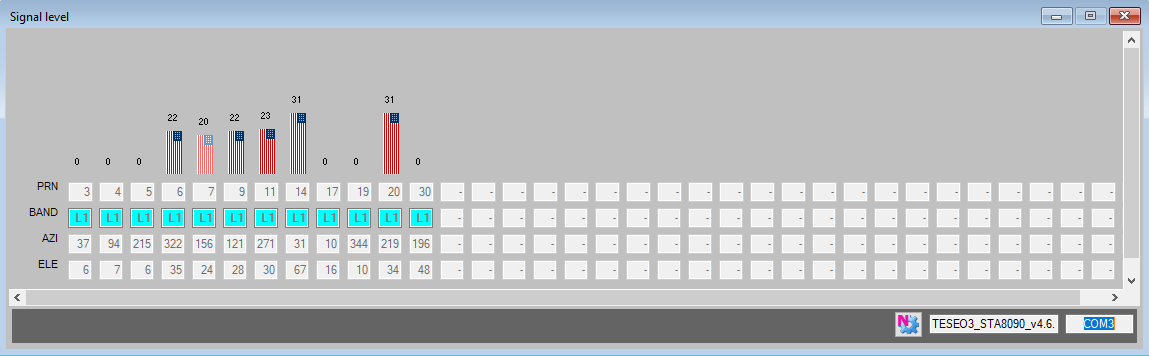
\includegraphics[width=14cm]{contents/chapter-3/setting-konstelasi/sebelum-konfigurasi.png}
 	\caption{Isyarat yang Digunakan oleh Teseo-LIV3FL Sehelum Konfigurasi}
 	\label{Fig: sebelum-konfigurasi}
 \end{figure}
 
Konfigurasi konstelasi yang akan digunakan dilakukan dengan membuka menu \textit{configuration wizzards} dan memilih opsi \textit{constellation}. Akan terbuka jendela baru berisi \textit{constellation} seperti ditunjukan oleh Gambar \ref{Fig: pilih-konstelasi}. Pada penelitian ini akan digunakan empat konstelasi, yaitu GPS, BeiDou, QZSS, dan Galileo.

\begin{figure}[H]
	\centering
	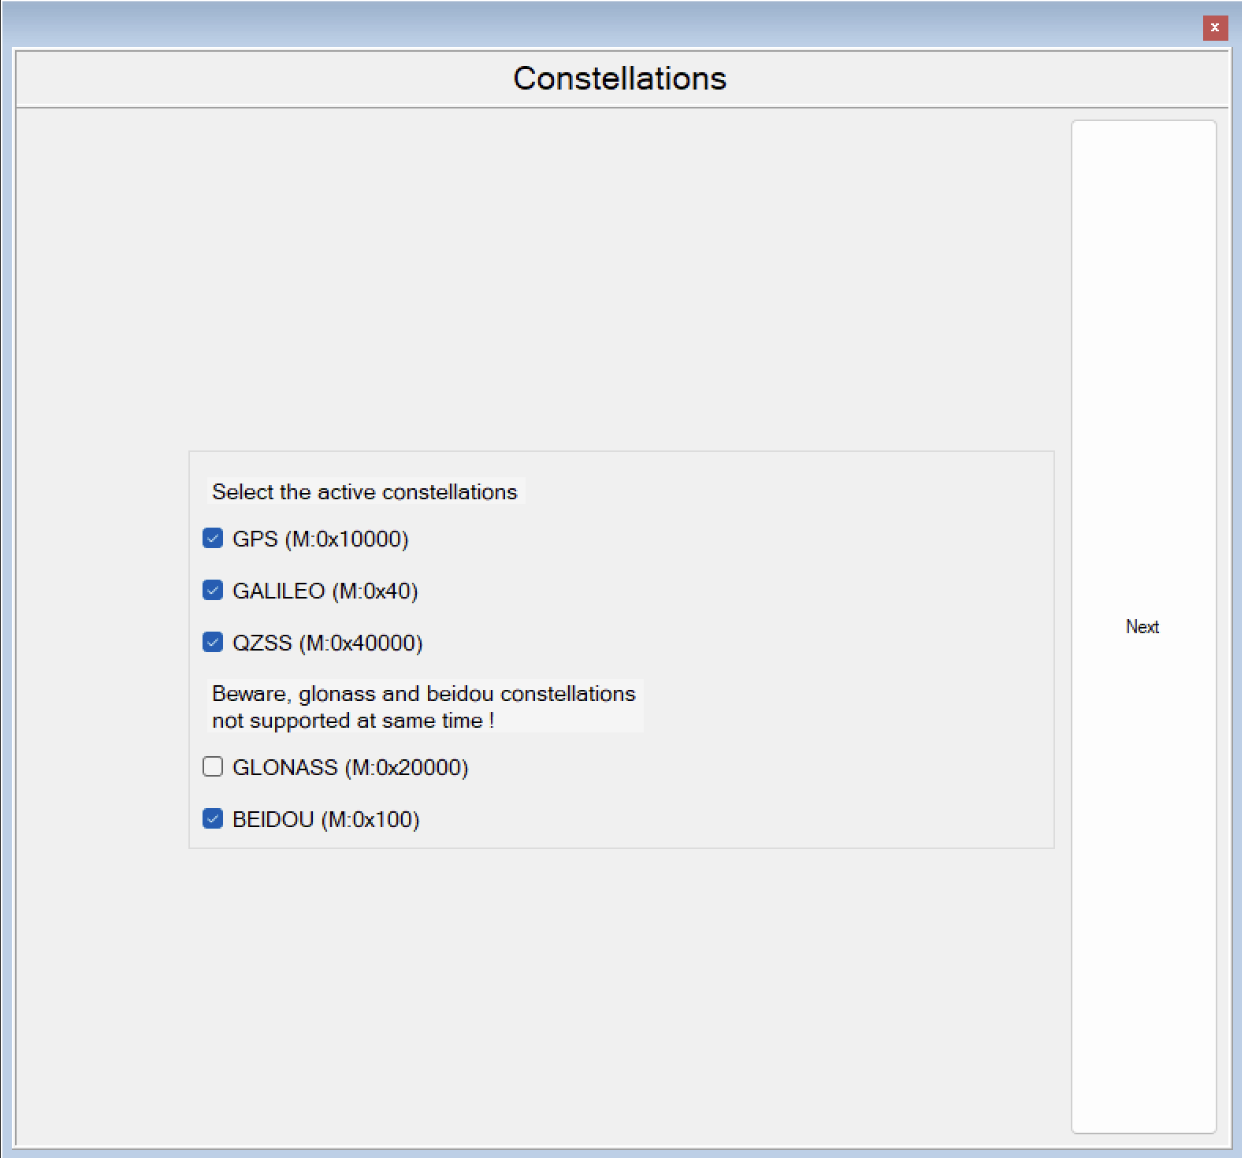
\includegraphics[width=10cm]{contents/chapter-3/setting-konstelasi/pilih-konfigurasi.png}
	\caption{Tampilan Pemilihan Konstelasi}
	\label{Fig: pilih-konstelasi}
\end{figure}


Lanhkah selanjutnya adalah klik tombol \textit{send my configuration to the device} seperti ditunjukan pada Gambar \ref{Fig: kirim-konstelasi}. Aplikasi Teseo-Suite akan mengirimkan perintah berikut ke modul GNSS.
\begin{verbatim}
	$PSTMSETPAR,1200,E70000
	$PSTMSETPAR,1200,C50000
	$PSTMSETPAR,1227,3C0
	$PSTMSAVEPAR
\end{verbatim}
Perintah tersebut akan mengubah  konfigurasi pada CDB-ID 200 dan CDB-ID 227. CDB-ID 200 berisi pengaturan untuk mengatur konstelasi GPS dan QZSS, sedangkan CDB-ID 227 untuk mengatur konstelasi BeiDou dan Galileo. Perintah \texttt{\$PSTMSAVEPAR} digunakan untuk menyimpan perubahan konfigurasi yang telah dilakukan.

\begin{figure}[H]
	\centering
	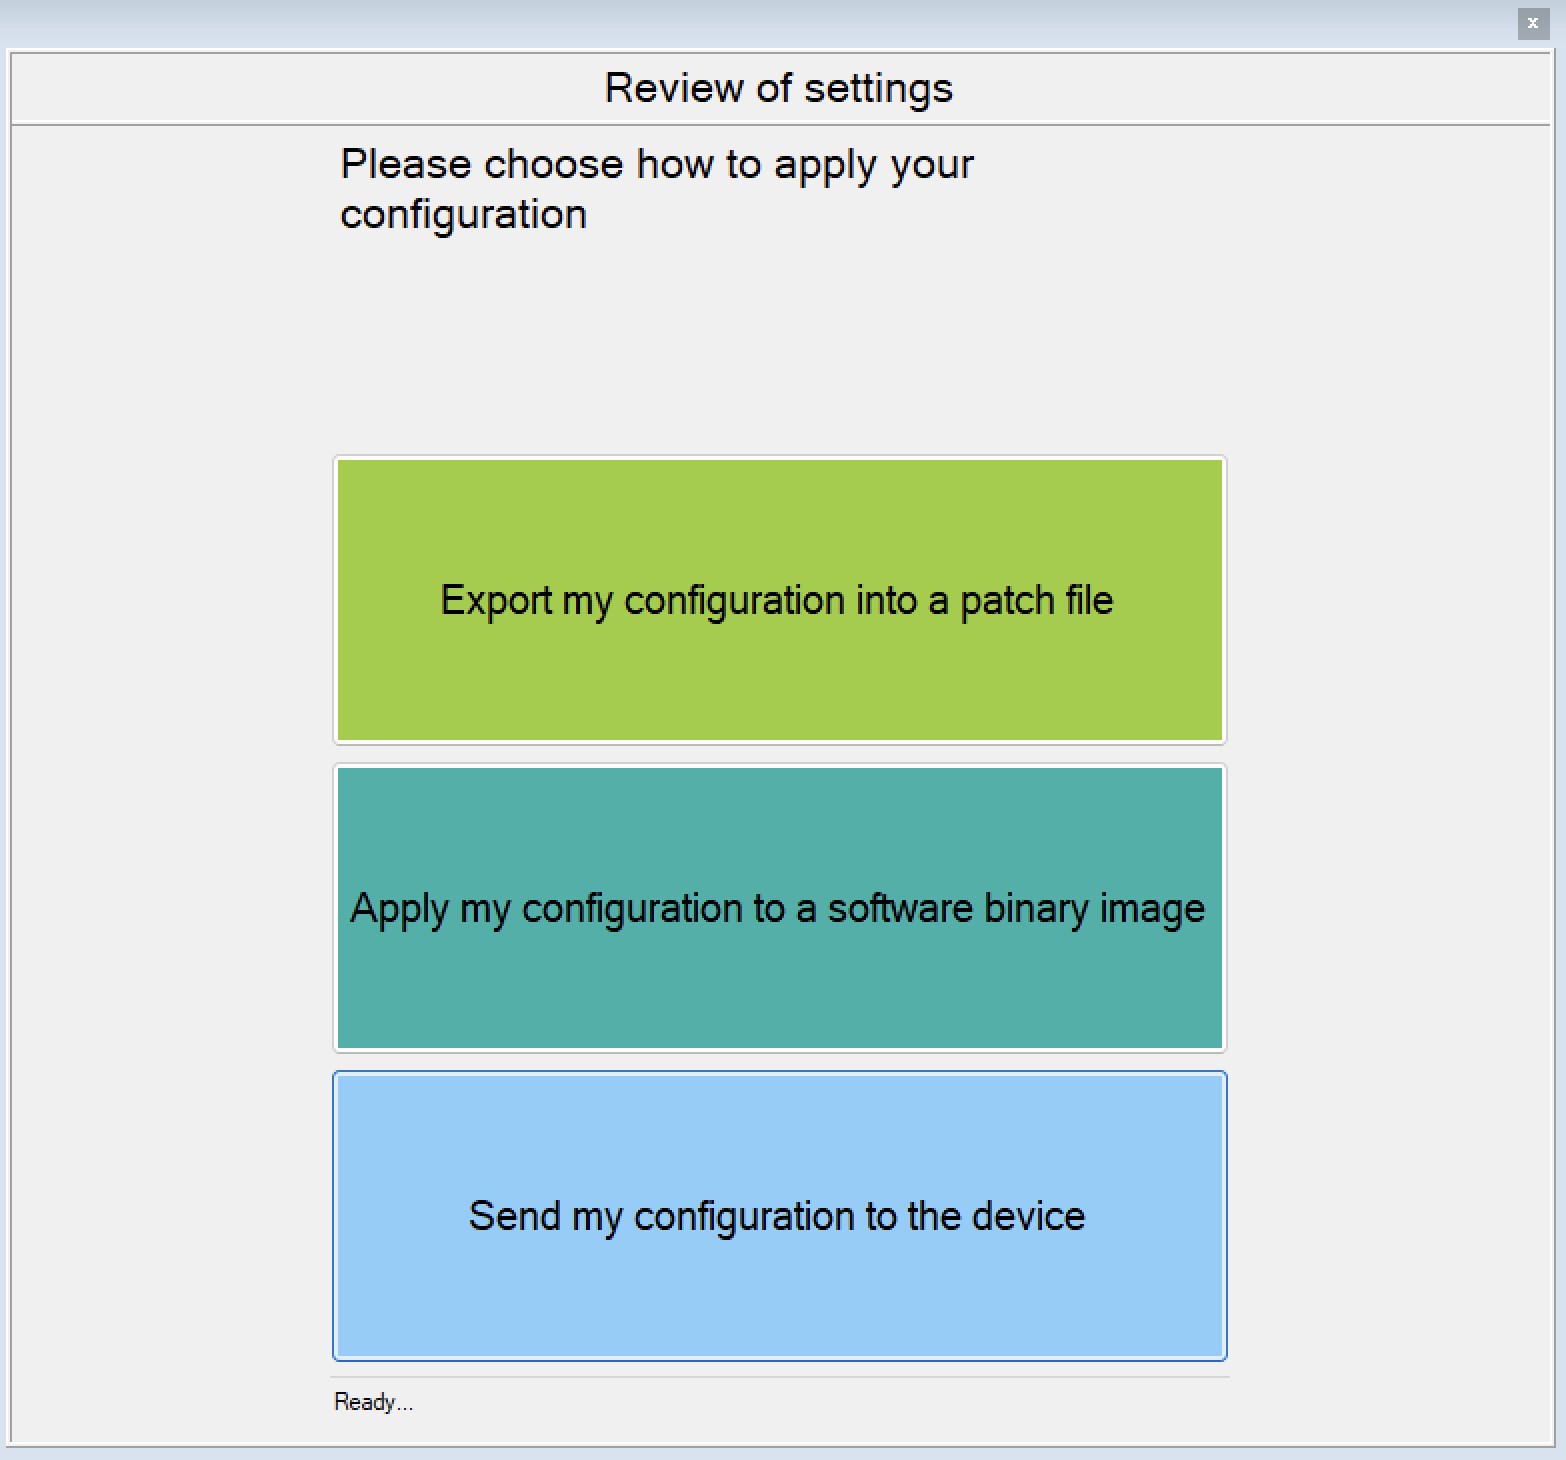
\includegraphics[width=10cm]{contents/chapter-3/setting-konstelasi/kirim-konfigurasi.png}
	\caption{Tampilan untuk Mengirim Konfigurasi}
	\label{Fig: kirim-konstelasi}
\end{figure}

Setelah konfigurasi sukses diunggah maka modul Teseo-LIV3FL akan menggunakan tiga konstelasi lain yang telah diaktifkan. Gambar \ref{Fig: setelah-konfigurasi} menunjukan bahwa modul Teseo-LIV3FL sudah menggunakan empat buah konstelasi, yaitu GPS, BeiDou, QZSS, dan Galileo.

\begin{figure}[H]
	\centering
	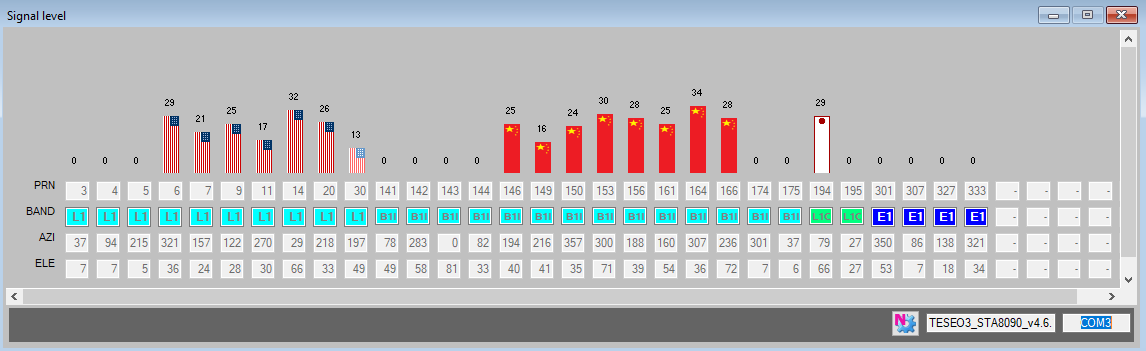
\includegraphics[width=14cm]{contents/chapter-3/setting-konstelasi/setelah-konfigurasi.png}
	\caption{Isyarat yang Digunakan oleh Teseo-LIV3FL Setelah Konfigurasi}
	\label{Fig: setelah-konfigurasi}
	\end{figure}

\section{Pengembangan \textit{Firmware} Mikrokontroler}
Pengembangan \textit{firmware} dilakukan dengan menggunakan STM32Cube IDE dan menggunakan bahasa pemrograman C. Untuk mempermudah pengembangan maka tahapan pengembangan dibagi menjadi tiga bagian kecil. Tiga bagian kecil tersebut tersebut adalah:
\begin{enumerate}
	\item Penguraian kalimat NMEA untuk ekstrasi data dari setiap kalimat NMEA yang digunakan
	\item Konversi koordinat dari bentuk \texttt{ddmm.mmm} ke derajat desimal untuk mempermudah proses selanjutnya
	\item Algoritma \textit{geofence} untuk menentukan apakah letak bus berada di dalam area kampus UGM atau tidak
\end{enumerate}
diagram alir \textit{firmware} secara garis besar ditunjukan oleh Gambar \ref{Fig: flowchart-firmware}.

\begin{figure}[H]
	\centering
	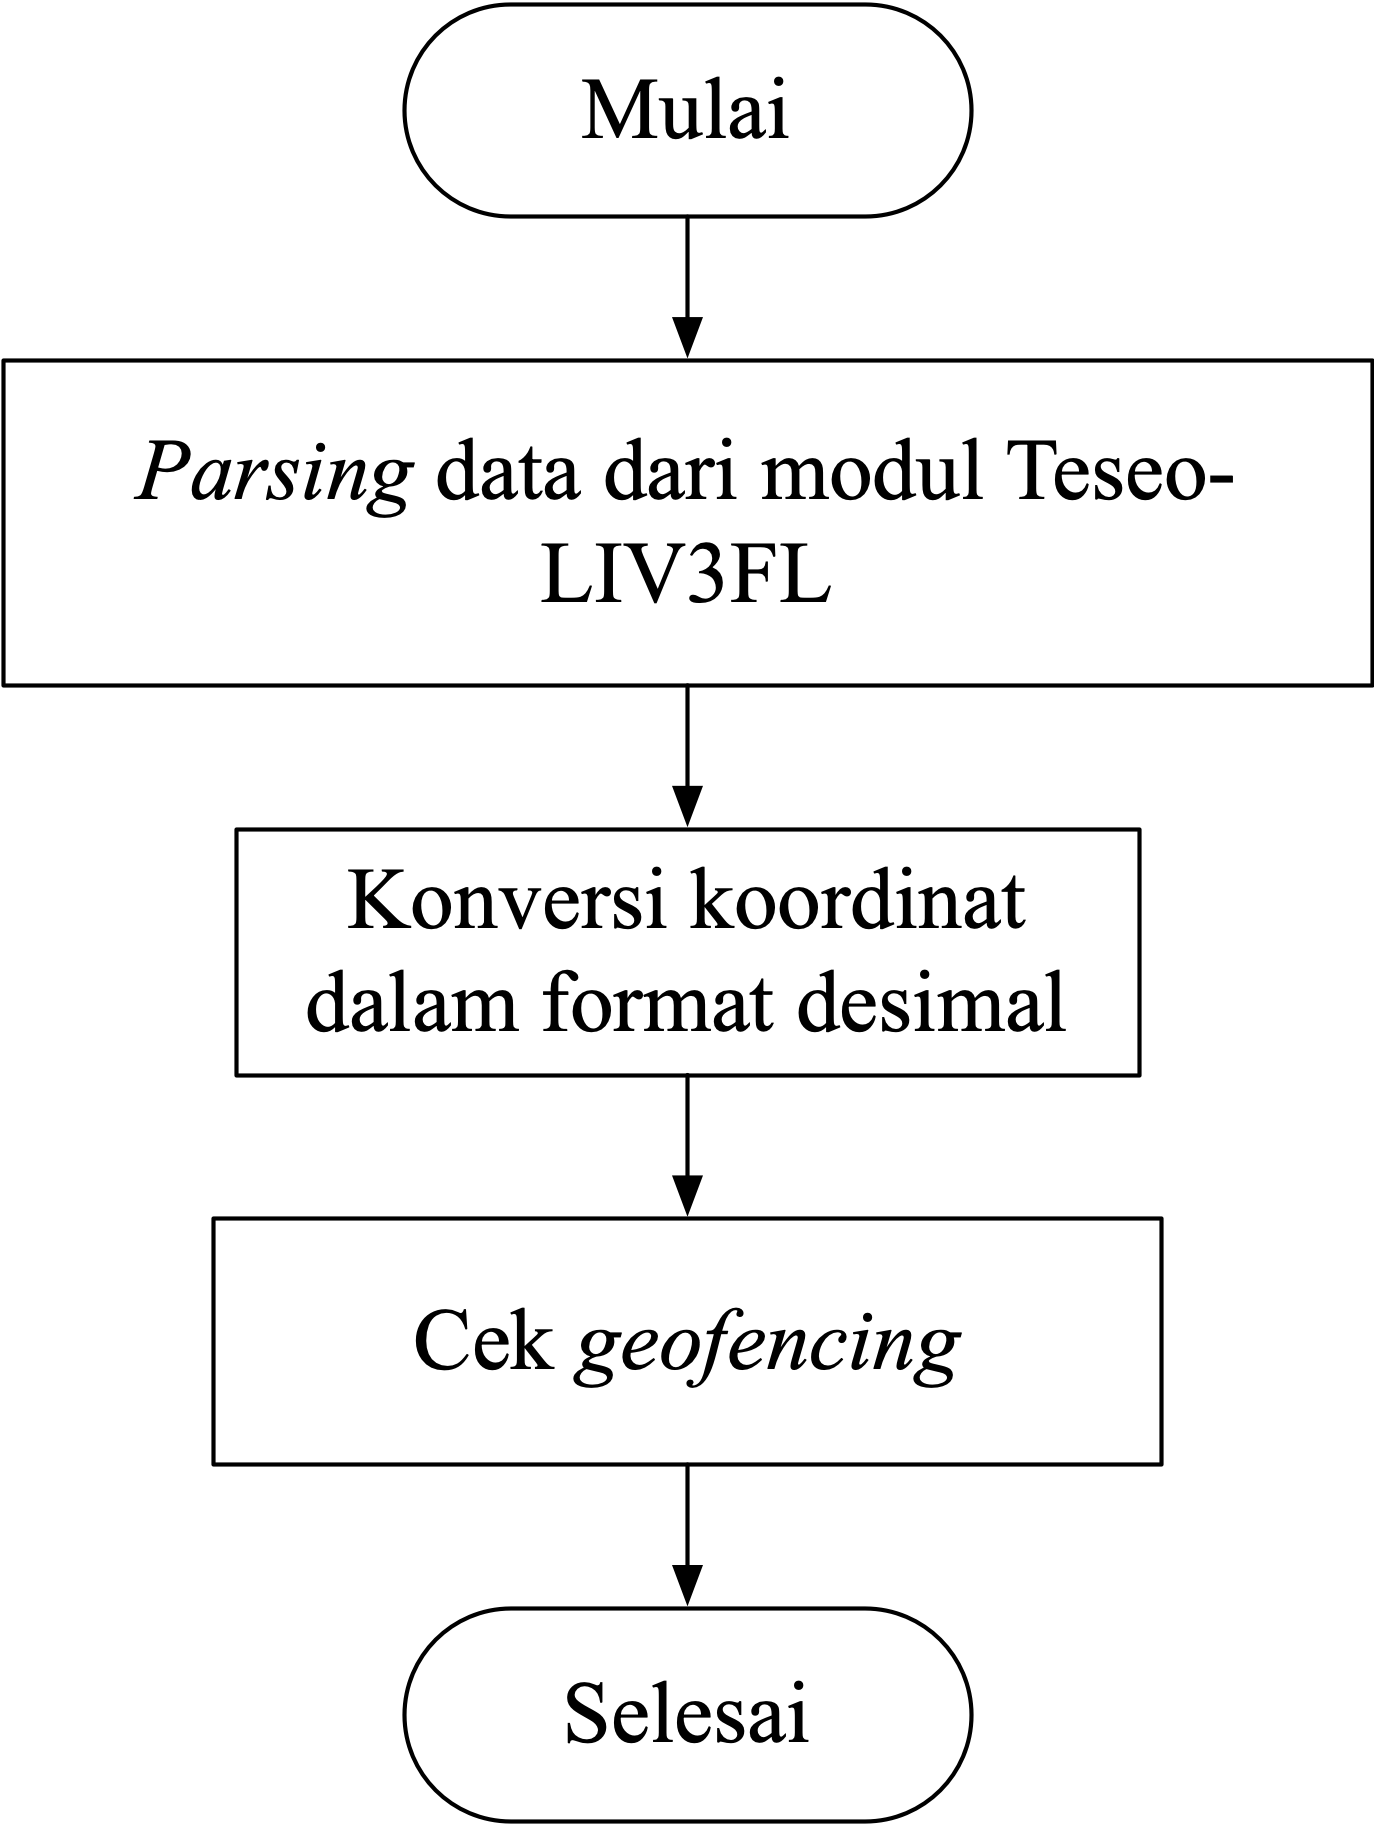
\includegraphics[width=6.3cm]{contents/chapter-3/firmware-diagram.png}
	\caption{Diagram Alir \textit{Firmware}}
	\label{Fig: flowchart-firmware}
\end{figure}


\subsection{Penguraian Kalimat NMEA}
Modul Teseo-LIV3FL mengirimkan data dengan mengikuti standar NMEA-0813 milik \textit{National Marine Electronics Association}. NMEA-0813 memiliki beberapa format data, tetapi pada penelitian ini hanya akan digunakan dua kalimat NMEA saja, yaitu GPGGA yang berisi data tetap GNSS dan GNGSA yang berisi nilai DOP dari pembacaan. Pada kalimat NMEA, setiap informasi dipisahkan oleh tanda koma dan asteris untuk memisahkan dengan \textit{checksum}. Struktur dari kalimat GNGSA dan GPGGA dengan struktur dari dua kalimat tersebut ditunjukan oleh oleh Tabel 3.1 dan Tabel 3.2.

\newpage

\begin{longtblr}[caption = {Struktur Pesan \$GNGSA}]{
		width = \linewidth,
		colspec = {Q[125]Q[817]},
		row{1} = {c},
		cell{2}{1} = {c},
		cell{3}{1} = {c},
		cell{4}{1} = {c},
		cell{5}{1} = {c},
		cell{6}{1} = {c},
		cell{7}{1} = {c},
		cell{8}{1} = {c},
		cell{9}{1} = {c},
		hline{1-2,10} = {-}{},
	}
	\textbf{Struktur} & \textbf{Deskripsi}                                                             \\
	header            & \textit{Header} pesan \\
	mode M/A          & A jika otomatis dan M jika dipaksa untuk peroperasi pada mode 2D atau 3D       \\
	mode 123          & 1 jika tidak ada \textit{fix}, 2 untuk mode 2D, dan 3 untuk mode 3D        \\
	prn               & ID satelit yang digunakan (kosong jika dalam mode \textit{multi-constellation} \\
	pdop              & Nilai PDOP                                                                     \\
	hdop              & Nilai HDOP                                                                     \\
	vdop              & Nilai VDOP                                                                     \\
	chksum            & \textit{Checksum}dalam bentuk heksadesimal
\end{longtblr}

\begin{longtblr}[caption = {Struktur Pesan \$GPGGA}]{
width = \linewidth,
colspec = {Q[98]Q[717]},
row{1} = {c},
cell{2}{1} = {c},
cell{2}{3} = {c},
cell{3}{1} = {c},
cell{3}{3} = {c},
cell{4}{1} = {c},
cell{4}{3} = {c},
cell{5}{1} = {c},
cell{5}{3} = {c},
cell{6}{1} = {c},
cell{6}{3} = {c},
cell{7}{1} = {c},
cell{7}{3} = {c},
cell{8}{1} = {c},
cell{8}{3} = {c},
cell{9}{1} = {c},
cell{9}{3} = {c},
cell{10}{1} = {c},
cell{10}{3} = {c},
cell{11}{1} = {c},
cell{11}{3} = {c},
cell{12}{1} = {c},
cell{12}{3} = {c},
cell{13}{1} = {c},
cell{13}{3} = {c},
cell{14}{1} = {c},
cell{14}{3} = {c},
cell{15}{1} = {c},
cell{15}{3} = {c},
cell{16}{1} = {c},
cell{16}{3} = {c},
cell{17}{1} = {c},
cell{17}{3} = {c},
hline{1-2, 18} = {-}{},
}
\textbf{Struktur}   & \textbf{Deskripsi} \\
\texttt{header}     & \textit{Header} pesan\\
\texttt{utc}        & Waktu UTC dalam format hhmmss.ss \\
\texttt{lat}        & Garis lintang\\
\texttt{lat\_dir}   & Arah garis lintang\\
\texttt{lon}        & Garis bujur \\
\texttt{lon\_dir}   & Arah garis bujur \\
\texttt{quality}    & Kualitas \textit{fix}. Jika bernilai nol maka tidak \textit{valid}\\
\texttt{satelit}    & Jumlah satelit yang digunakan\\
\texttt{hdop}       & Nilai HDOP \\
\texttt{alt}        & Ketinggian antena dari permukaan laut\\
\texttt{a-units}    & Satuan dari ketinggian antena\\
\texttt{und} & Perbedaan ketinggian antara Geoid dengan elipsoid \\
\texttt{u-units}    & Satuan dari perbedaan ketinggian\\
\texttt{age}        & Umur dari koreksi data dalam sekon (kosong jika tidak ada data diferensial) \\
\texttt{stn-ID}     & Nomor pengidentifikasi stasiun referensi differensial (kosong jika tidak ada data diferensial)\\
\texttt{chksum}     & \textit{Checksum} dalam bentuk heksadesimal   
\end{longtblr}

Secara garis besar, proses penguraian dibagi menjadi , yaitu inisiasi perangkat GNSS dan variabel penyimban hasil penguraian, akuisisi data dari modul Teseo-LIV3FL, cek \textit{sanity} untuk memeriksa integritas data yang diterima, proses penguraian utama, dan diakhiri dengan \textit{release} \textit{buffer} kalimat NMEA. Diagram alir proses penguraian ditunjukan oleh Gambar \ref{Fig: flowchart-parsing}.

\begin{figure}[H]
	\centering
	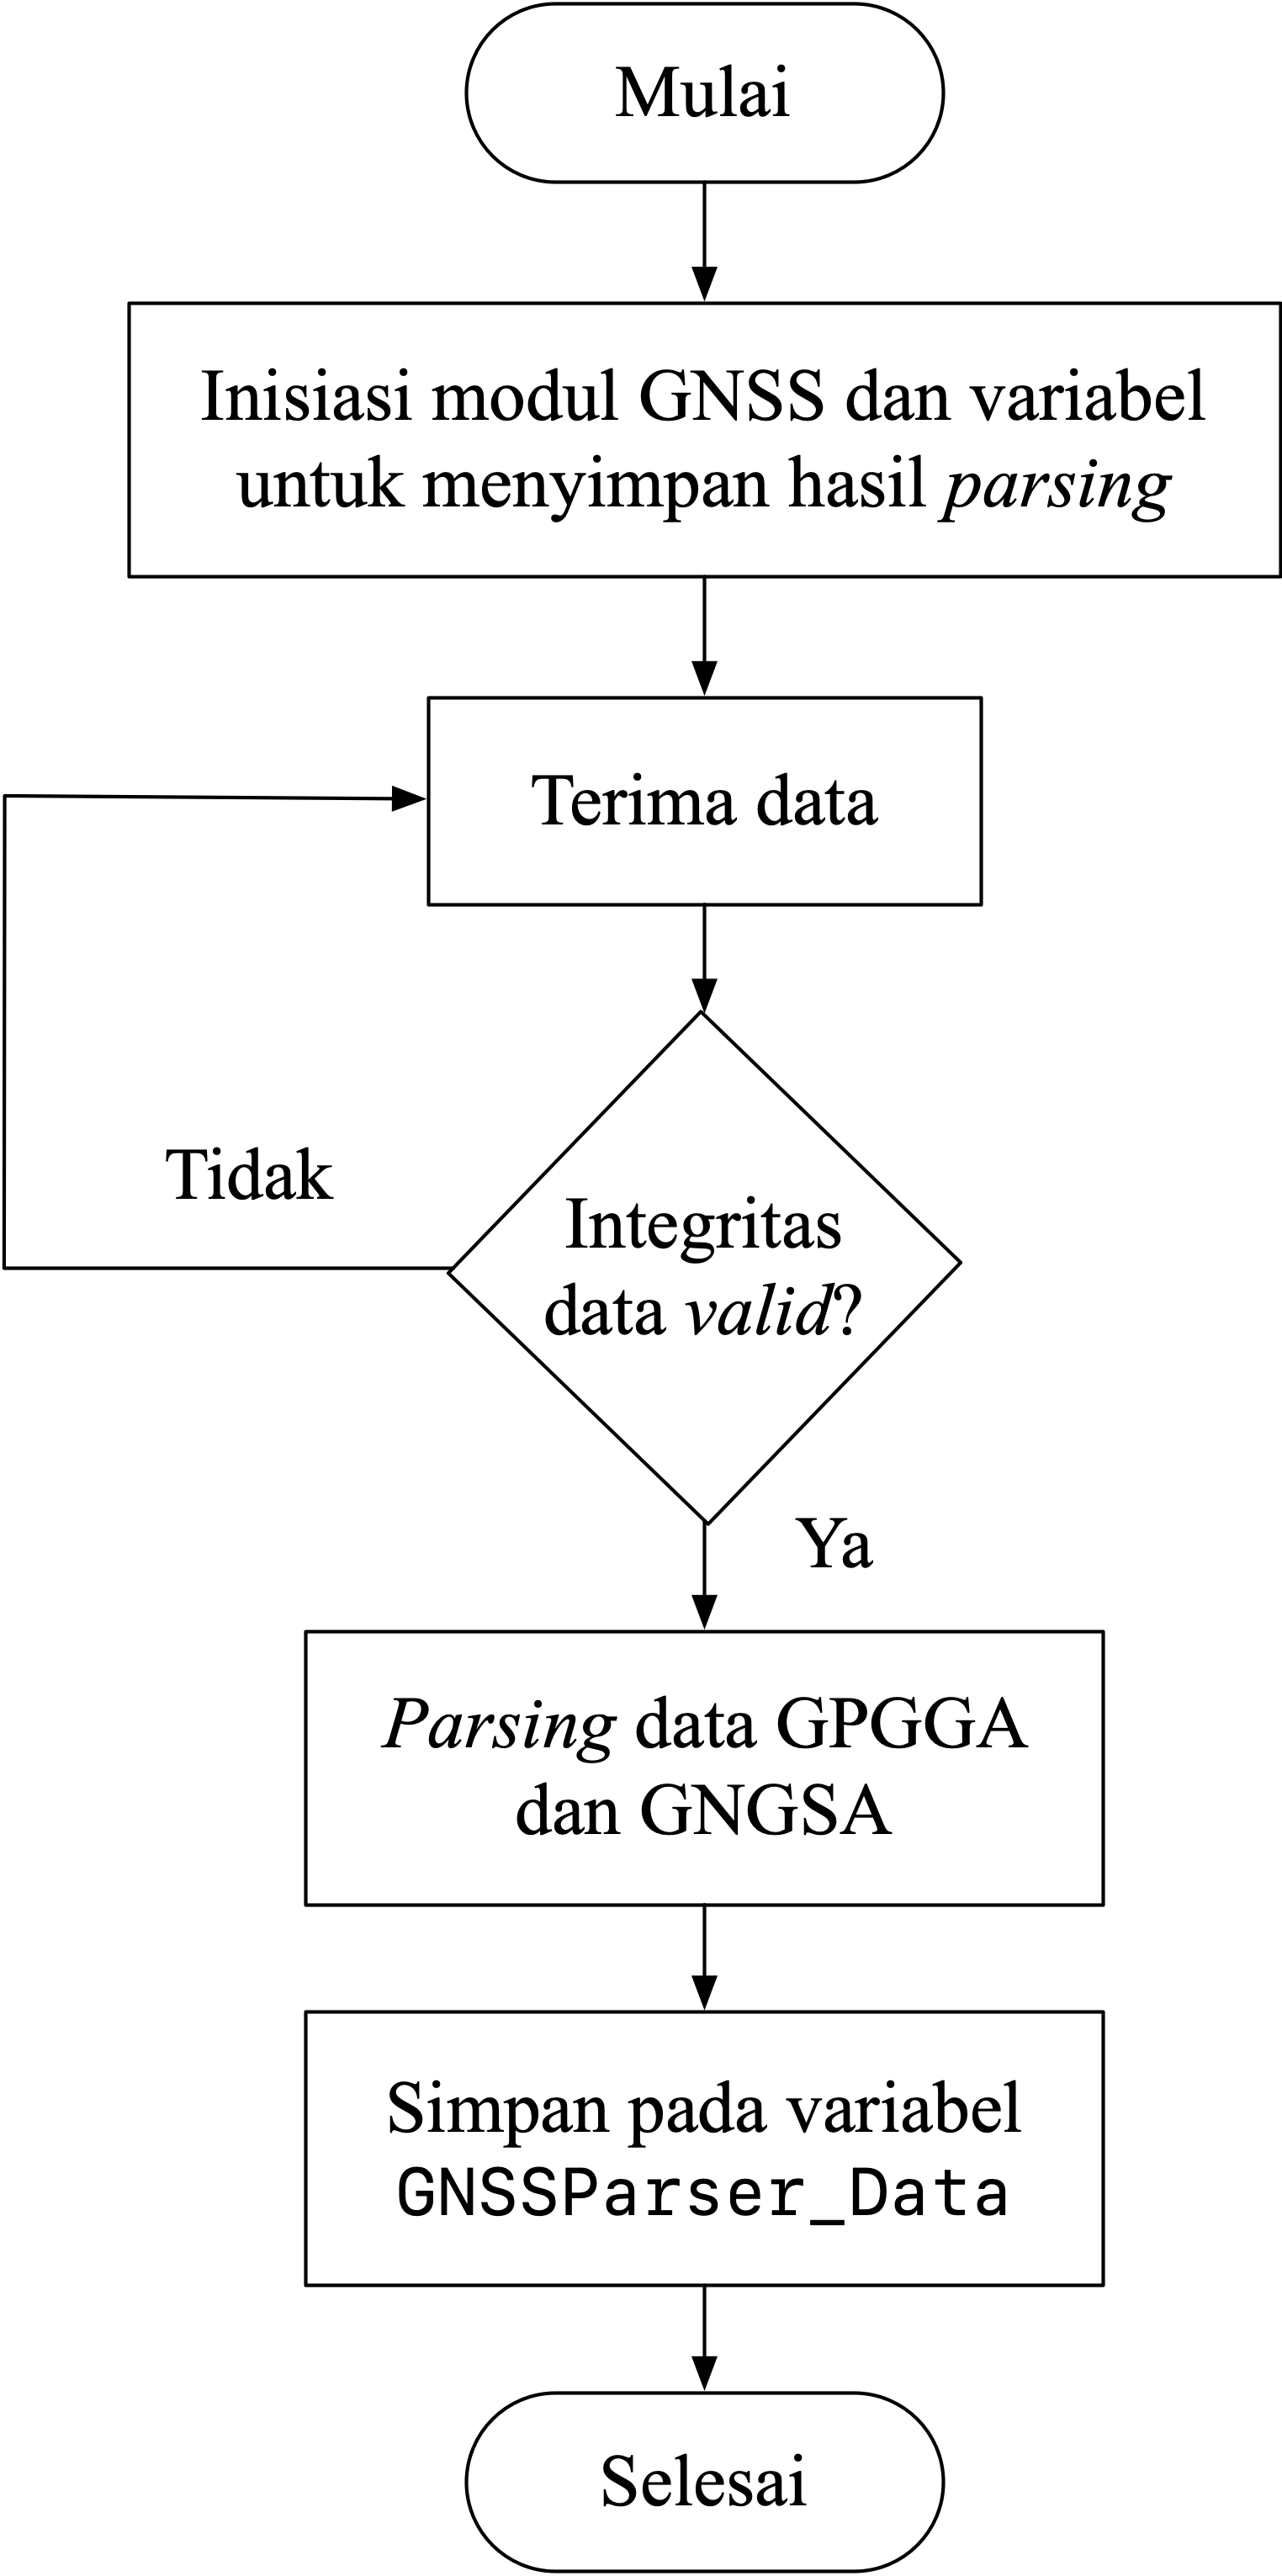
\includegraphics[width=6.5cm]{contents/chapter-3/diagram-parser.png}
	\caption{Diagram Alir Proses Penguraian Kalimat NMEA}
	\label{Fig: flowchart-parsing}
\end{figure}

\subsubsection{Inisiasi}
Proses penguraian diawali dengan melakukan inisiasi perangkat GNSS dan variabel untuk menyimpan data hasil penguraian dengan memanggil fungsi \texttt{CUSTOM\_GNSS\_Init} dan \texttt{GNSS\_PARSER\_Init}. 

Fungsi \texttt{CUSTOM\_GNSS\_Init} akan mengembalikan nilai dari variabel \texttt{ret}. Setelah itu, fungsi ini akan memanggil \texttt{TESEO\_LIV3F\_Probe()} untuk memeriksa apakah modul Teseo-LIV3FL sudah terhubung dengan baik atau tidak. Jika modul GNSS sudah terhubung dengan baik maka fungsi akan mengembalikan nilai \texttt{BSP\_ERROR\_NONE}, sedangkan jika terdapat galat pada modul maka fungsi akan mengembalikan nilai \texttt{BSP\_ERROR\_NO\_INIT}.

Selanjutnya, fungsi  \texttt{CUSTOM\_GNSS\_Init} dipanggil untuk inisiasi struktur \texttt{GNSSParser\_Data\_t}. Pada fungsi ini, struktur \texttt{gpgga\_data} dan \texttt{gsa\_data} diatur menjadi nol untuk menghindari galat atau hal tidak terduga lainnya. Jika proses inisiasi struktur berjalan dengan lancar maka fungsi akan mengembalikan \texttt{GNSS\_PARSER\_OK} dan \texttt{GNSS\_PARSER\_ERROR} jika terdapat galat.

Setelah inisiasi berhasil proses selanjutnya adalah menerima data yang dikirimkan oleh modul Teseo-LIV3FL dengan memanggil fungsi \texttt{CUSTOM\_GNSS\_GetMessage} dan disimpan pada variabel \texttt{gnssMsg} yang berisi nilai dari \textit{buffer} dan panjangnya.

\subsubsection{Cek Integritas Data}
Pesan yang diterima tidak selalu dalam keadaan sempurna. Sebagai contoh, terdapat sebagian karakter pada pesan yang hilang atau tercampur dengan karakter lainnya. Untuk memastikan bahwa pesan yang didapat adalah benar maka digunakan fungsi \texttt{GNSS\_PARSER\_CheckSanity} untuk memeriksa integritas data yang diterima. 

Sebelum melakukan proses pengecekan, nilai \textit{checksum} dari kalimat NMEA masih dalam bentuk heksadesimal sehingga perlu dilakukan konversi ke bentuk integer terlebih dahulu.

Proses pengecekan dilakukan dengan membandingkan \textit{checksum} data yang diterima dengan yang tertera pada kalimat NMEA. \textit{Checksum} dilakukan dengan mengenakan operasi XOR pada setiap \textit{bytes} di antara simbol "\$" dan "*". Jika hasil \textit{checksum} pada kalimat NMEA sama dengan hasil perhitungan maka fungsi akan mengembalikan \texttt{GNSS\_PARSER\_OK}. Sebaliknya, jika hasil \textit{checksum} berbeda maka fungsi akan mengembalikan \texttt{GNS\_PARSER\_ERROR}.

Potongan kode sumber di bawah menunjukan fungsi \texttt{GNSS\_PARSER\_CheckSanity} untuk proses pengecekan integritas data dari kalimat NMEA.
\begin{lstlisting}[language=c]
checksum = (char2int(pSentence[len-4U]) << 4) | char2int(pSentence[len-3U]);
		
for(uint64_t c = 1U; c < (len-5U); c++) {
	check = (check ^ pSentence[c]);
}
		
ret = (check == checksum) ? GNSS_PARSER_OK : GNSS_PARSER_ERROR;
	
return ret;
\end{lstlisting}

\subsubsection{Proses Penguraian Utama}
Modul GNSS Teseo-LIV3FL mengirimkan tiga belas kalimat NMEA standar dan empat kalimat NMEA milik STMicroelectronics yang diawali oleh \$PSTM. Karena pada penelitian hanya digunakan kalimat GPGGA dan GNGSA maka diperlukan suatu mekanisme untuk memeriksa apakah kalimat yang diterima termasuk di antara salah satu yang digunakan. Proses penguraian kalimat GPGGA dan GNGSA dibuat dalam dua fungsi yang berbeda untuk mempermudah pengembangan. 

Fungsi \texttt{NMEA\_ParseGPGGA} digunakan untuk menguraikan kalimat GPGGA. Variabel \texttt{app} diinisiasikan sebagai larik yang berisi \textit{string}. Bagian perulangan dilakukan hingga \textit{line break} atau karakter \texttt{\textbackslash n}. Setelah perulangan selesai variabel \texttt{app} akan berisi seluruh bagian yang terdapat pada kalimat NMEA. 

Variabel \texttt{i} digunakan sebagai indeks dari perulangan, sedangkan \texttt{j} dan \texttt{k} sebagai indeks dari variabel \texttt{app}. Nilai \texttt{valid\_msg} akan bernilai benar jika kalimat NMEA yang diterima diawali dengan \$GPGGA. Sebaliknya, perulangan akan dihentikan jika pesan NMEA yang diterima tidak diawali dengan  \$GPGGA.

Jika karakter pada iterasi saat ini adalah asteris atau tanda koma maka karakter terakhir akan diatur sebagai \textit{null terminator}. Selain itu, variabel \texttt{k} akan diatur kembali menjadi nol dan \texttt{j} ditambahkan satu. Sebaliknya, jika karakter pada iterasi saat ini bukan asteris atau tanda koma maka karakter tersebut akan disimpan dalam variabel \texttt{app} dengan indeks \texttt{j} dan \texttt{k}. Bagian perulangan ditunjukan oleh kode sumber di bawah

\begin{lstlisting}[language=c]
for (int32_t i = 0, j = 0, k = 0; (NMEA[i] != (uint8_t)'\n'); i++)
{
	new_field = 0;
	
	if ((NMEA[i] == (uint8_t)',') || (NMEA[i] == (uint8_t)'*'))
	{
		app[j][k] = (uint8_t)'\0';
		new_field = 1;
		
		if (strcmp((char *)app[0], "$GNGSA") == 0)
		{
			j++;
			k = 0;
			valid_msg = TRUE;
		}
		else
		{
			break;
		}
	}
	if(new_field == 0)
	{
		app[j][k] = NMEA[i];
		k++;
	}
}
\end{lstlisting}

Hasil akhir dari perulangan di atas masih dalam bentuk tipe data \textit{string}, sedangkat beberapa data yang dibutuhkan harus dalam berbentuk angka. Untuk menyelesaikan masalah tersebut maka harus dilakukan konversi tipe data dari \textit{string} menjadi tipe data yang diinginkan. Digunakan fungsi standar C \texttt{strtod} untuk konversi ke \textit{double floating point}, \texttt{strtof} untuk konversi ke \textit{floating point}, dan \texttt{strtol} untuk konversi ke \textit{long integer}. Proses konversi ditunjukan pada kode sumber di bawah
\begin{lstlisting}[language=c]
pGPGGAInfo->xyz.lat = strtod((char *)app[2], NULL);
pGPGGAInfo->xyz.lon = strtod((char *)app[4], NULL);
pGPGGAInfo->sats = strtol((char *)app[7], NULL, BASE);
pGPGGAInfo->acc = strtof((char *)app[8], NULL);
pGPGGAInfo->xyz.alt = strtof((char *)app[9], NULL);
pGPGGAInfo->geoid.height = strtol((char *)app[11], NULL, BASE);
\end{lstlisting}

Fungsi \texttt{scan\_utc} dikembangkan untuk mengolah data waktu UTC yang disimpan dalam format \texttt{hhmmss.sss}. Adapun data yang diambil adalah nilai jam, menit, dan detik. Nilai jam dihitung dengan membagi variabel \texttt{utc} dengan 10000, kemudian nilai menit dihitung dengan mengurangi hasil kali nilai jam dengan 10000 dari variabel \texttt{utc} dan membaginya dengan 100, dan nilai detik dihitung dengan mengurangi variabel \texttt{utc} dengan hasil kali nilai jam dengan 10000 dan hasil kali nilai menit dengan 100. Implementasi dari fungsi \texttt{scan\_utc} ditunjukan oleh kode sumber di bawah
\begin{lstlisting}[language=c]
static void scan_utc(uint8_t *pUTCStr, UTC_Info_t *pUTC)
{
	pUTC->utc = strtol((char *)pUTCStr,NULL,10);
	
	pUTC->hh = (pUTC->utc / 10000);
	pUTC->mm = (pUTC->utc - (pUTC->hh * 10000)) / 100;
	pUTC->ss = pUTC->utc - ((pUTC->hh * 10000) + (pUTC->mm * 100));
	
	return;
}
\end{lstlisting}

Proses penguraian kalimat GNGSA hampir sama dengan proses penguraian kalimat GPGGA. Perbedaan antara dua fungsi tersebut hanya data apa saja yang diurai dari dua kalimat tersebut. Seluruh hasil penguraian data akan disimpan dalam variabel \texttt{GNSSParser\_Data}.

\subsection{Konversi Koordinat}
Koordinat yang didapat dari proses penguraian pada bagian sebelumnya masih dalam bentuk \texttt{ddmm.mm} dengan dua digit pertama adalah derajat dan empat digit lainnya adalah menit. Untuk mempermudah visualisasi dan perhitungan pada algoritma \textit{geofencing} maka perlu dikonversi terlebih dahulu ke bentuk derajat desimal. Konversi dapat dilakukan dengan menggunakan persamaan berikut

\begin{equation}
	dd = deg + \frac{min}{60} 
\end{equation}
Jika arah dari koordinat garis lintang berada di bagian selatan (S) maka hasil konversi dikalikan dengan -1. Hal yang sama juga dilakukan jika arah dari koordinat garis bujur berada di bagian barat (W).

Konversi koordinat pada \textit{firmware} berada di dalam fungsi \texttt{Convert\_to\_Degree}. Fungsi ini menerima argumen \texttt{numeral} dengan tipe data \textit{floating point} dalam format \texttt{ddmm.mmm} dan argumen \texttt{sign} sebagai arah dari koordinat hasil penguraian. Implementasi dari fungsi \texttt{Convert\_to\_Degree} ditunjukan oleh kode sumber di bawah
\begin{lstlisting}[language=c]
float64_t Convert_to_Degree(float64_t numeral, uint8_t sign) {
	int32_t degrees;
	float64_t ret;
	float64_t minutes;
	
	degrees = (int32_t) (numeral / 100.0F);
	minutes = numeral - degrees * 100.0F;
	ret = degrees + (minutes / 60.0F);
	
	if (sign == 'S' || sign == 'W') {
		ret = -ret;
	}
	
	return ret;
}
\end{lstlisting}

Hal pertama yang dilakukan oleh fungsi ini adalah melakukan konversi bagian derajat dengan membagi \texttt{numeral} dengan seribu dan di-\textit{cast} ke tipe data \textit{integer}. Hasil perhitungan disimpan di dalam variabel \texttt{degrees}.

Untuk menghitung bagian menit maka nilai koordinat asal dikurangi \texttt{degrees} dikalikan dengan seratus. Hasil yang didapat adalah bagian menit yang kemudian disimpan dalam variabel \texttt{minutes}.

Setelah mendapatkan bagian menit dan derajat, maka hasil akhirnya adalah hasil penjumlahan dari \texttt{degrees} ditambah dengan hasil pembagian \texttt{minutes} dengan enam puluh. Operasi pembagian dilakukan karena terdapat enam puluh menit dalam satu derajat. Hasil perhitungan akan disimpan dalam variabel \texttt{ret}.

Terakhir, fungsi akan memeriksa arah dari koordinat dalam variabel \texttt{sign}. Jika nilai dari \texttt{sign} adalah S atau W maka hasil akhir koordinat akan dinegasikan atau dikalikan dengan negatif satu. Hal tersebut dikarenakan selatan dan barat berada di bagian negatif sistem koordinat standar. Fungsi akan mengembalikan nilai \texttt{ret} yang berupa \textit{floating point}.

\subsection{Algoritma \textit{Geofencing}}
Komputasi \textit{geofencing} dilakukan pada sisi mikrokontroler dengan menggunakan fungsi \texttt{Geofence\_Check()}. Fungsi ini membutuhkan dua buah argumen, yaitu \texttt{latitude} untuk koordinat garis lintang dan \texttt{longitude} untuk koordinat garis bujur. Kedua argumen dalam bentuk \textit{floating point}. Fungsi ini akan mengembalikan \textit{integer} untuk menunjukan apakah koordinat yang diberikan berada di dalam lingkaran dari satu titik yang telah ditentukan. Pada penelitian ini, titik pusat lingkaran diatur pada koordinat (-7.771376, 110.377493) dengan jari-jari 1000 m seperti ditunjukan oleh daerah yang ditutupi oleh lingkaran hitam pada Gambar  \ref{Fig: geofence-map}.

\begin{figure}[H]
	\centering
	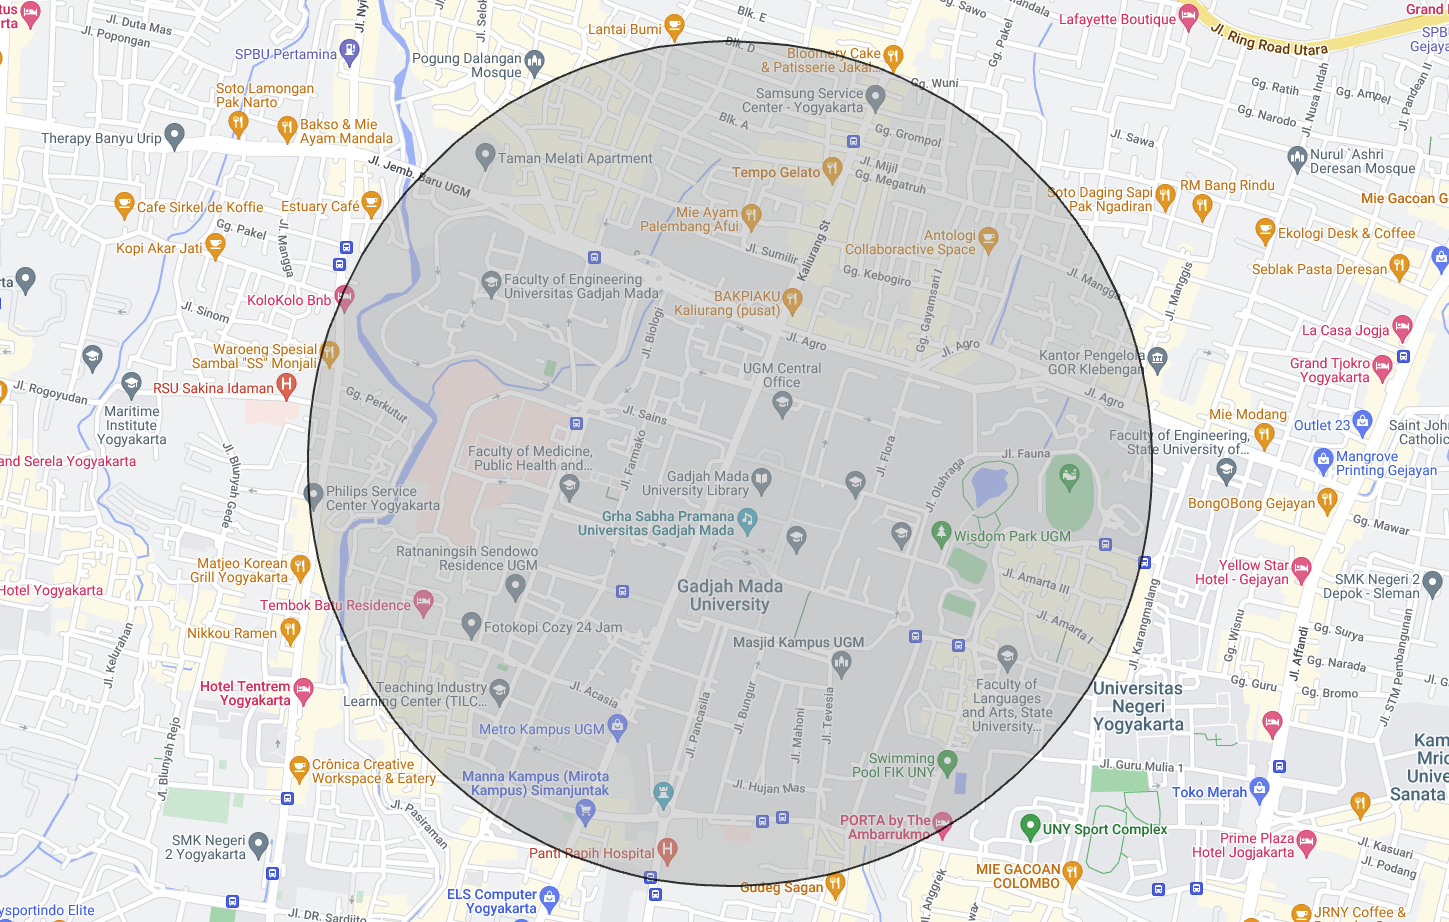
\includegraphics[width=12cm]{contents/chapter-3/geofence-map.png}
	\caption{Daerah \textit{Geofencing}}
	\label{Fig: geofence-map}
\end{figure}

Tahap pertama yang dilakukan adalah inisiasi struktur \texttt{ugm\_coordinate} berisi koordinat dari titik pusat lingkaran dan variabel \texttt{distance} untuk menyimpan perhitungan jarak. Potongan kode sumber di bawah menunjukan inisiasi koordinat titik pusat.
\begin{lstlisting}[language=c]
Coords_t ugm_coordinate;
float64_t distance = 0;

ugm_coordinate.lat = -7.771376;
ugm_coordinate.lon = 110.377493;
\end{lstlisting}

Selanjutnya, selisih dari koordinat garis bujur dan garis lintang disimpan pada variabel \texttt{dLon} dan \texttt{dLat} seperti ditunjukan pada potongan kode sumber di bawah
\begin{lstlisting}[language=c]
float64_t dLat = degToRad(ugm_coordinate.lat) - degToRad(latitude);
float64_t dLon = degToRad(ugm_coordinate.lon) - degToRad(longitude);
\end{lstlisting}
Karena fungsi trigonometri dari pustaka \texttt{math.h} menerima argumen dalam satuan radian maka kedua nilai tersebut akan dikonversi dari derajat ke radian dengan fungsi yang telah didefinisikan sebelumnya.
\begin{lstlisting}[language=c]
#define degToRad(angleInDegrees) ((angleInDegrees) * M_PI / 180.0)
\end{lstlisting}

Kemudian, akan digunakan persamaan Haversine untuk menghitung jarak antara dua titik pada permukaan bola. Setelah itu, hasil perhitungan akan dikalikan dengan jari-jari bumi dan disimpan pada variabel \texttt{distance}. Implementasi dari persamaan Haversine ditunjukan oleh potongan kode di bawah
\begin{lstlisting}[language=c]
float64_t a = pow(sin(dLat / 2), 2) + pow(sin(dLon / 2), 2) * cos(latitude) * cos(longitude);
float64_t c = 2 * asin(sqrt(a));
\end{lstlisting}

Terakhir, fungsi ini akan memeriksa apakah jarak yang telah di hitung kurang dari jarak \textit{geofence} atau tidak. Jika jarak antar dua titik kurang dari jarak \textit{geofence} maka fungsi akan mengembalikan nilai satu sebagai representasi bahwa titik berada di dalam lingkaran dan nilai nol jika sebaliknya. Potongan kode di bawah menunjukan proses pengecekan jarak antara dua titik
\begin{lstlisting}[language=c]
 if (distance < 1000) {
	return 1;
} else {
	return 0;
}
\end{lstlisting}